% SplitMem manuscript (IEEEtran journal format). Build: python -I <skill>/scripts/compile.py main.tex --export "SplitMem.pdf" --png pages
% Every table body in tables/ is generated by make_tables.py from the raw result files; figures by make_figures.py.
\documentclass[journal]{IEEEtran}
\usepackage[T1]{fontenc}
\usepackage{amsmath,amssymb}
\usepackage{mathptmx}
\usepackage{graphicx}
\usepackage{multirow}
\usepackage{array}
\usepackage{cite}
\usepackage{url}
\usepackage{microtype}
\usepackage{xcolor}
\usepackage{algorithm}
\usepackage[noend]{algpseudocode}
\renewcommand{\algorithmicrequire}{\textbf{Input:}}
\renewcommand{\algorithmicensure}{\textbf{Output:}}
\usepackage{placeins}
\renewcommand{\arraystretch}{1.12}\setcounter{topnumber}{3}
\setcounter{dbltopnumber}{3}
\setcounter{totalnumber}{5}
\renewcommand{\topfraction}{0.9}
\renewcommand{\dbltopfraction}{0.9}
\renewcommand{\textfraction}{0.08}
\renewcommand{\floatpagefraction}{0.75}
\renewcommand{\dblfloatpagefraction}{0.75}

\title{SplitMem: Split Cloud-Edge Forecasting\\ With Node Memory for Low-Cost PM Sensor Nodes}
\author{Samiul Seikh, Suyash Kumar, and Kartik%
\thanks{The authors are with the Netaji Subhas University of Technology, New Delhi, India. Department and e-mail addresses to be added.}}

\begin{document}
\maketitle

\begin{abstract}
Low-cost particulate matter (PM) sensor nodes can densely cover a city, but each node sees only its own surroundings and runs on a microcontroller that cannot hold a large forecasting model. Training a small on-device model to copy a large cloud model gave little here, because the large model is better mainly through information the node never receives. In this work, we propose SplitMem, a cloud-assisted on-device forecaster that sends the missing information to the node instead of trying to teach it. Specifically, the cloud uses the uploads of all nodes to forecast the shared city-wide change of PM2.5 and PM10 and broadcasts it in eight bytes per hour, and the node model predicts only its own local difference. A node memory, a table of 48 numbers that stores how far the node usually sits above or below the city at each clock hour, adds a second component with no link cost. On simulated nodes at 32 Delhi-NCR stations, driven by real CPCB and ERA5 data from 2018 to 2026, the stack raises the 1 to 3 h forecast skill over persistence from 16.0\% to 18.9\% at known places and from 17.5\% to 21.1\% at five places never used in training, about 3.4\% and 4.3\% lower RMSE. A placebo that reads another node's table recovers one sixth of the memory gain. A disagreement-triggered personal cloud forecast recovers two thirds of the full cloud gain with one fifth of the messages. Wind direction, a learned send rule and a buffered broadcast fail, and robustness to stale links costs accuracy. All sensors are simulated.
\end{abstract}

\begin{IEEEkeywords}
Air quality forecasting, low-cost sensors, edge computing, cloud-edge collaboration, particulate matter, TinyML.
\end{IEEEkeywords}

\section{Introduction}
\IEEEPARstart{F}{ine} particulate matter (PM2.5 and PM10) is the pollutant that drives the air quality index in Delhi for most of the year, and a forecast of its change over the next few hours lets people and authorities act before a peak arrives. Official monitoring stations are accurate but few, so many projects now place low-cost sensor nodes, built around an ESP32 microcontroller with a PM sensor and a few gas and weather sensors, across a city \cite{an2025gta,illueca2024zoning}. A node of this kind should still give a useful forecast when its network link is slow, expensive, or down.

Two facts make this hard. First, the node sees only its own place. In a city where one weather regime moves most stations together, a single node sees a noisy copy of a signal that many neighbours measure better. Second, the node must run on a few hundred kilobytes of memory, so the models that forecast best, graph and transformer networks \cite{qi2026bernt,dimri2026transnet,wang2024wddstg}, cannot run on it. The usual answer in edge forecasting is to train a small model to imitate a large one \cite{hinton2015distill,na2026privileged,fu2026rednet,kumar2026kdaqnet}. That answer works when the large model sees the same inputs and is simply bigger. It is less suitable when the large model is better because it sees other places, since the small model cannot reproduce what it never observes.

We met this limit directly. In our first design, a cloud graph model that sees all nodes scored a skill of 20.8\% against 15.0\% for the on-device model, and training the on-device model to match the cloud model added only 0.9 points. The gap is an information gap, not a capacity gap. This observation changes the design question from ``how do we squeeze the cloud model into the node'' to ``which few bytes of what the cloud knows should the node receive, and what should the node do with them''.

In this work, we propose SplitMem, a cloud-assisted on-device forecaster. It is not a compressed copy of a cloud model: the cloud and the node run different models on different inputs and predict different quantities. The cloud forecasts the common, city-wide change of PM and broadcasts it in eight bytes per hour. The node predicts only its own local difference from that broadcast, which we call the local correction, and it keeps a small memory of its own habits. Because the node output is a difference from a shared forecast, the design resembles common-mode rejection in electronics: everything the nodes share is subtracted, and the small model spends its few parameters on what only this node can see.

Our contributions are summarized below.
\begin{itemize}
\item We propose a split cloud-edge forecaster in which the cloud broadcasts a city-wide change forecast in eight bytes and the on-device model predicts only the local correction. It lowers the RMSE by 1.58\% (95\% CI $-1.90$ to $-1.27$) against the same node model working alone, and raises the skill at new places from 17.5\% to 19.9\%.
\item We introduce node memory, a per-clock-hour table of the node's offset from the broadcast level with 48 stored numbers and no extra link bytes. A placebo-controlled test shows the gain is specific to the node: the real table lowers RMSE by 1.09\% (CI $-1.27$ to $-0.91$) beyond the split model, and another node's table gives about one sixth of it.
\item We show, with matched comparisons, why copying a cloud model into the node gave little here, and we give a rule for what to send instead. We measure the cost of sending personal cloud forecasts only when the cloud and the node disagree.
\item We report the negative results of the project with the same care as the positive ones: wind direction, a physics block, custom losses, a learned send rule, a buffered broadcast, and training for stale links.
\end{itemize}

All sensor values in this study come from a physics-based simulator of the node, driven by real station data. We therefore present the numbers as evidence that the design is worth building, not as the performance of a deployed device.

Section~\ref{sec:related} reviews related work. Section~\ref{sec:method} describes SplitMem. Section~\ref{sec:exp} reports the experiments, Section~\ref{sec:discussion} analyses the results and the limits, and Section~\ref{sec:conclusion} concludes.

\section{Related Work}
\label{sec:related}
\subsection{Graph and Transformer Models for Air Quality Forecasting}
Most recent work on multi-station forecasting uses a graph over the stations and an attention-based temporal encoder. ST-BernT combines a Bernstein-polynomial graph filter, built from distance and from correlation between pollutant series, with a transformer for multisite prediction \cite{qi2026bernt}. Several models make the graph depend on the wind: WDDSTG-Net builds a dynamic directed graph from the wind direction for ozone \cite{wang2024wddstg}, and WSDST-GAT combines a wind-aware graph, a transformer encoder and co-kriging for the same pollutant in Beijing \cite{wu2026wsdst}. A dynamic geographical graph adds terrain and landform to the distance graph for PM2.5 \cite{zhao2025dggnn}. TransNet learns advection, diffusion and reaction operators to forecast PM2.5 up to 72 h ahead across South Korea \cite{dimri2026transnet}, and TopoFlow adds topography-aware attention to a vision transformer for high-resolution prediction \cite{kheder2026topoflow}. These models run in the cloud on data from all stations and report accuracy on station networks. They do not consider a node that must produce its own forecast with a small model, and they do not test the physical prior against a control. We include a graph model of this kind as the cloud part of our system, and we test its wind prior against a rotated-wind placebo.

\subsection{Low-Cost Sensors and Virtual Sensing}
Low-cost PM sensors are biased by humidity and need calibration, and networks of them are often combined with a few reference stations. Virtual sensing estimates PM2.5 where no sensor exists from nearby sensors, using a mechanistic humidity correction and a graph-transformer model on a LoRa and oneM2M platform \cite{an2025gta}. Neural networks can calibrate the output of a chemistry-transport model with hyperlocal measurements for air quality zoning \cite{illueca2024zoning}, and mobility data from cameras and traffic sensors improves graph-based prediction of traffic-related pollutants \cite{morales2025mobility}. These works estimate or predict with the cloud as the place of computation. We instead ask what a single node can do on its own, and how few bytes from the cloud improve it.

\subsection{Lightweight Forecasting and Knowledge Distillation}
Lightweight forecasters trade accuracy for cost, for example by decoupling a series into feature maps for long-term forecasting \cite{tang2025tsm}. Knowledge distillation \cite{hinton2015distill} trains a small student to match a large teacher and is the standard tool for edge forecasting. For on-device forecasting, a transformer teacher guides a student built from gated dilated depthwise convolutions, using information that is available to the teacher during training \cite{na2026privileged}. REDNet distils a large pre-trained foundation forecaster into a small edge model in two stages, aiming at stable output under noisy or corrupted input \cite{fu2026rednet}. KDAQnet distils a satellite-based multi-pollutant forecaster \cite{kumar2026kdaqnet}, and a gradient boosting model can act as the teacher of a symbolic regression student \cite{shmuel2026forest}. In these works the teacher and the student either see the same series or the teacher receives extra data only during training. Our teacher-like cloud model sees other nodes at run time, which the node cannot, and the measured gain from copying it is small. We adopt the compact student architecture of \cite{na2026privileged} for the on-device model, but we feed it network information as an input rather than as a training target. The idea of a global forecast corrected by a local model is also common in forecasting practice; our contribution is its form for byte-limited links and microcontroller models, the node memory, and the measurements at known and new places.

\section{Methodology}
\label{sec:method}
\subsection{Overview}
Fig.~\ref{fig:framework} shows SplitMem. Every hour each node uploads its 23 sensor features. The cloud stacks the uploads of all $N$ nodes and runs two models. The regional branch averages the nodes' own PM readings and forecasts the city-wide change of $\ln$ PM for the next three hours. The result, together with the current regional level, is broadcast to all nodes in eight bytes plus one sequence byte. The graph branch, a cloud graph model, forecasts each node separately; its output is used only for personal forecasts, which the cloud sends to a node when it disagrees with what the node is predicted to say. The node combines its own last 24 hours, the broadcast, and a state derived from its history (consensus level and memory) in a small convolutional model whose output is the broadcast forecast plus a local correction.

\begin{figure*}[!t]
\centering
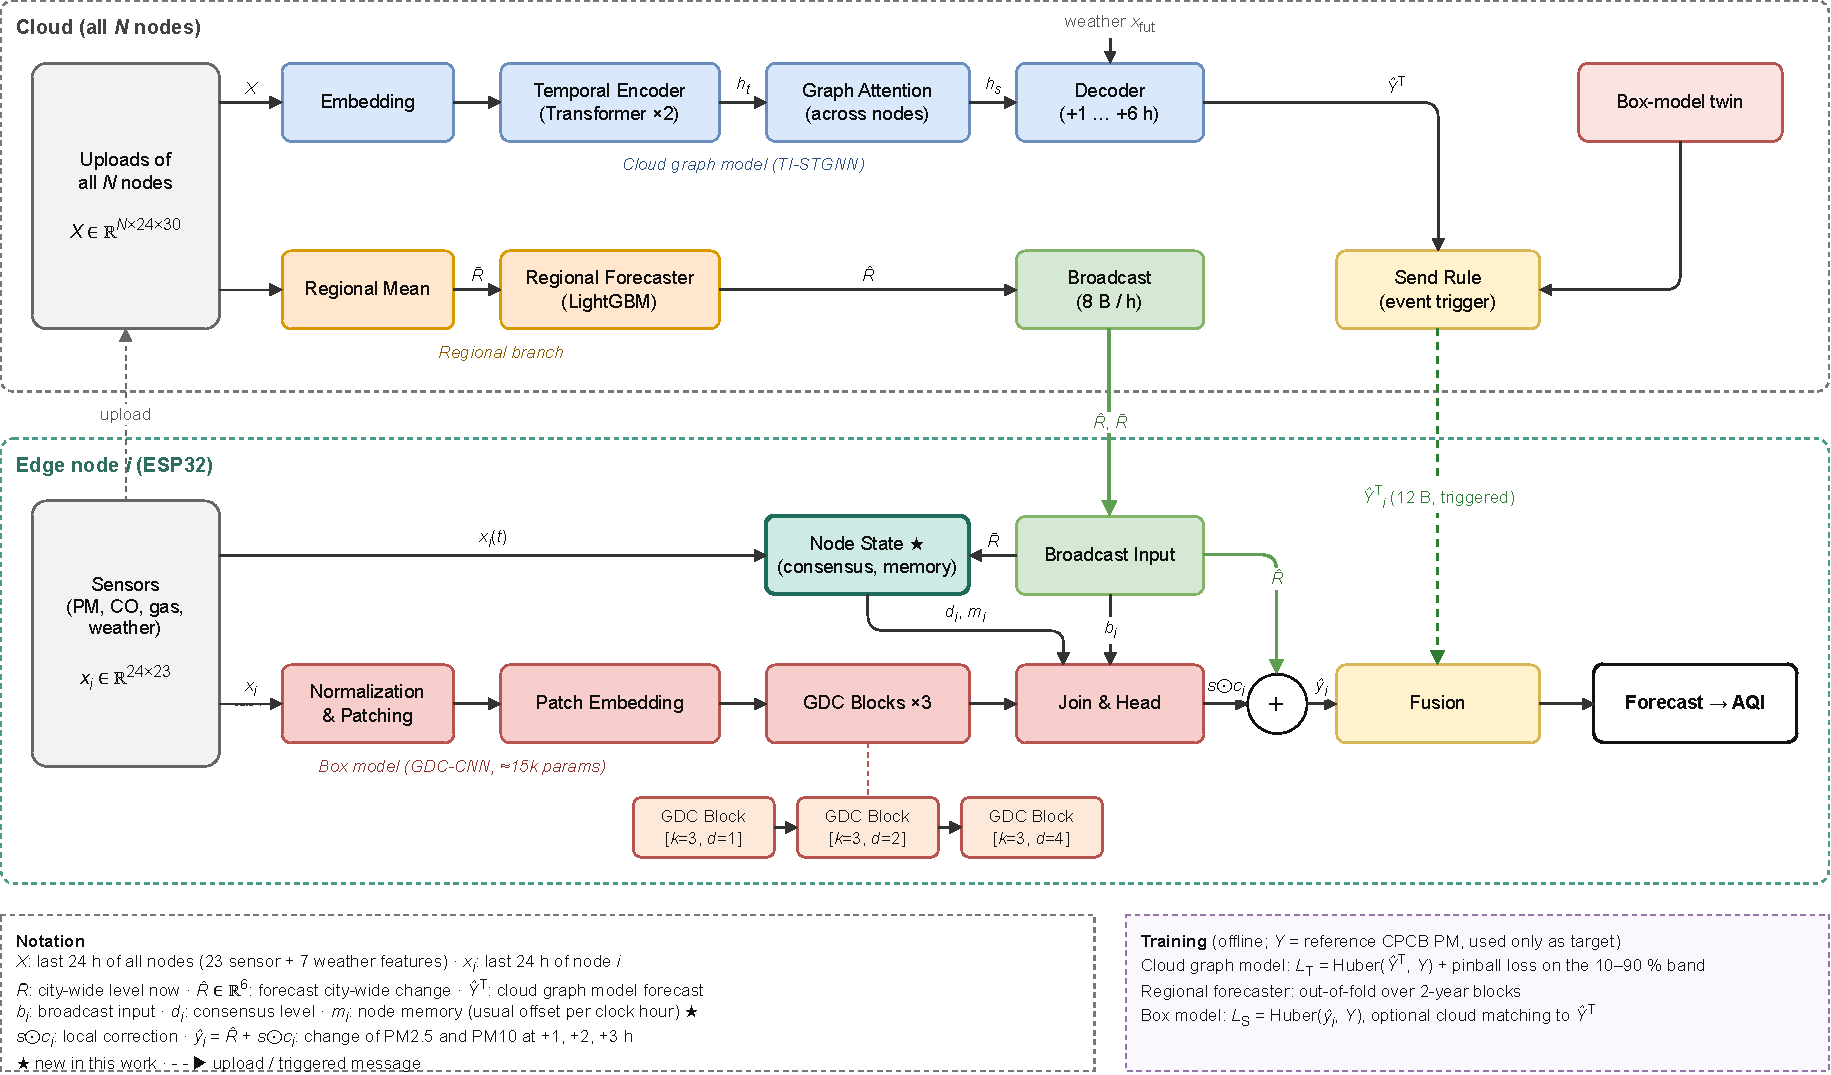
\includegraphics[width=\textwidth]{figures/fig1_architecture.pdf}
\caption{Overall framework of SplitMem. The cloud (top) forecasts the shared change from all nodes and broadcasts it in eight bytes per hour; the cloud graph model produces personal forecasts that are sent only when it disagrees with a twin of the node model. The node (bottom) predicts its local correction on top of the broadcast, using a node state made of the consensus level and the node memory (marked with a star, new in this work). Dashed arrows are the upload and the triggered personal message.}
\label{fig:framework}
\end{figure*}

\subsection{Problem Definition}
Let $\mathrm{PM}^p_i(t)$ be the reference concentration of pollutant $p \in \{2.5, 10\}$ at the place of node $i$ in clock hour $t$. The node forecasts the change
\begin{equation}
y^p_{i,h}(t) = \ln\!\big(1+\mathrm{PM}^p_i(t+h)\big) - \ln\!\big(1+\mathrm{PM}^p_i(t)\big),\quad h=1,2,3,
\label{eq:target}
\end{equation}
which gives six outputs $[y^{2.5}_{1..3}, y^{10}_{1..3}]$. We forecast the change and not the level because the level of a low-cost sensor is biased by humidity and calibration, while its change is much less so. The level shown to a user comes from calibration against a reference station and from the cloud. The inputs of every model are simulated node features only: the reference PM serves as the target and never as an input, for the node or for its neighbours. The score is the skill over persistence,
\begin{equation}
\text{skill} = 1 - \frac{\mathrm{RMSE}(\hat y, y)}{\mathrm{RMSE}(0, y)} ,
\label{eq:skill}
\end{equation}
where persistence ($\hat y=0$) means that PM stays unchanged. Skill 0 is no better than that baseline.

\subsection{Cloud Regional Forecaster and Broadcast}
Let $S^p_i(t)$ be the logarithm of the PM reading of node $i$. The regional level is the mean over the nodes that reported,
\begin{equation}
R^p(t) = \frac{1}{|\mathcal{N}_t|}\sum_{i\in\mathcal{N}_t} S^p_i(t).
\label{eq:region}
\end{equation}
A regional forecaster, one LightGBM model \cite{ke2017lightgbm} per output, maps a 36-number feature row to the city-mean change $\hat R_{h}^p$. The row holds $R^{2.5}$ and $R^{10}$ at lags of 0, 1, 2, 3, 6, 12 and 23 h with their 1 h and 3 h changes, the regional means of humidity, temperature, CO sensor and fan wind speed, the city-mean ERA5 weather now \cite{hersbach2020era5}, and clock features. Its target is the mean of the true changes over the nodes. To keep the node model from being trained on forecasts that have seen its own training hours, the forecaster is trained out-of-fold over three two-year blocks of the training years. Averaging many noisy nodes cancels the sensor noise of each one, so the city-wide change is easy for the cloud and hard for a single node. The broadcast carries $\hat R \in \mathbb{R}^6$ and the two levels $R^{2.5}(t), R^{10}(t)$ as signed bytes, eight bytes in total, plus one sequence byte that lets the node know the age of the message. On the node it becomes the broadcast input
\begin{equation}
\mathbf{b}_i(t) = \big[\,3\hat R,\; R^{2.5}(t)-S^{2.5}_i(t),\; R^{10}(t)-S^{10}_i(t)\,\big]\in\mathbb{R}^{8}.
\label{eq:broadcast}
\end{equation}

\subsection{On-Device Model With a Local Correction}
The on-device model is a gated dilated convolutional network in the style of \cite{na2026privileged}. Its 24 h input window $[24, 23]$ is normalised per feature by its own mean and standard deviation, which are kept: the standard deviation of $\ln$ PM2.5 and $\ln$ PM10 forms the scale $\mathbf{s}\in\mathbb{R}^6$. Two consecutive hours form a patch, giving $[12, 46]$, which a dense layer maps to width 32 with a learned position code. Three gated blocks with dilations 1, 2 and 4 follow; each block is a layer normalisation, a causal depthwise convolution with kernel 3, a dense layer with a gated linear unit \cite{dauphin2017glu}, and a residual connection. The block output is flattened to 384 numbers. Four side inputs enter through their own small dense layers: the raw regime context that normalisation removes (log PM2.5, humidity, temperature, CO sensor, clock and season terms, wind speed), the broadcast of (\ref{eq:broadcast}), the consensus state, and the memory state. Table~\ref{tab:layers} lists the shapes. The model has 14\,790 parameters for the context-only form and about 300 more for the side inputs, so it converts to a FP32 TensorFlow Lite model of a few tens of kilobytes.

\begin{table}[!htb]
\caption{Layers and Output Shapes of the On-Device Model}
\label{tab:layers}
\centering\footnotesize
\setlength{\tabcolsep}{3pt}
\begin{tabular}{|p{1.5cm}|p{4.5cm}|c|}
\hline
Stage & Operation & Output \\
\hline
Normalisation & per-feature mean and std, keep $\mathbf{s}$ & $[24,23]$ \\
Patches & 2 consecutive hours side by side & $[12,46]$ \\
Embedding & Dense 46$\to$32 + position code & $[12,32]$ \\
Blocks $\times3$ & LayerNorm, causal depthwise conv ($k{=}3$, $d{=}1,2,4$), Dense 64 + GLU, Dense 32, residual & $[12,32]$ \\
Flatten & & $[384]$ \\
Side inputs & four Dense 32 + GELU: context $[9]$, broadcast $[8]$, consensus $[3]$, memory $[8]$ & $4\times[32]$ \\
Head & concatenate $[512]$, Dense 512$\to$6, times $\mathbf{s}$ & $[6]$ \\
\hline
\end{tabular}
\end{table}

The output of the head is a correction, and the forecast is
\begin{equation}
\hat y_i(t) = \hat R(t) + \mathbf{s}\odot g\big(\mathbf{x}_i,\mathbf{b}_i,\mathbf{c}_i,\mathbf{m}_i\big),
\label{eq:split}
\end{equation}
where $\mathbf{x}_i$ is the window with its context, $\mathbf{c}_i$ the consensus state and $\mathbf{m}_i$ the memory state defined next. The network is trained against the node's own true targets with a Huber loss \cite{huber1964robust}. No cloud output is used as a training target in the main design.

\subsection{Consensus Level}
Averaging sensor networks smooths a node's reading towards its neighbours \cite{olfati2007consensus}. We estimate the node level as the region now plus the node's slow offset,
\begin{equation}
d_i(t) = R(t) + \mathrm{EWMA}_{24\,\mathrm{h}}\big(S_i - R\big)(t-1),
\label{eq:consensus}
\end{equation}
with an exponential moving average of half-life 24 h. This removes short sensor noise and keeps the persistent local offset. The consensus state is $\mathbf{c}_i=[\,d_i-S_i,\;3\Delta_{1\mathrm{h}}d_i,\;3\Delta_{3\mathrm{h}}d_i\,]$ for PM2.5.

\subsection{Node Memory}
The consensus level holds one average offset and does not know the clock. Local sources such as traffic peaks and evening burning repeat at the same hours every day and differ from site to site. The node therefore keeps, for each of the 24 clock hours $c$ and each pollutant, an exponentially weighted average over past days of its offset from the broadcast level,
\begin{equation}
o_i(t)=S_i(t)-R(t),\quad M_i(c_t)\leftarrow \lambda M_i(c_t)+(1-\lambda)\,o_i(t),
\label{eq:memory}
\end{equation}
with $c_t=\mathrm{clock}(t)$ and $\lambda=2^{-1/10}$, a half-life of ten days. The table has $24\times2=48$ numbers. Two kinds of input are derived from it,
\begin{equation}
\begin{split}
u_i(t)&=o_i(t)-M_i(c_t),\\
q_{i,h}(t)&=M_i(c_{t+h})-M_i(c_t),
\end{split}
\label{eq:surprise}
\end{equation}
the surprise, how unusual the node is now, and the profile, how its offset usually moves over the next one to three hours ($h=1,2,3$, scaled by 3). With two pollutants this gives eight inputs $\mathbf{m}_i=[u^{2.5}_i,u^{10}_i,q_{i,1..3}^{2.5},q_{i,1..3}^{10}]$. The entry for hour $t{+}h$ was last updated at $t{+}h{-}24$, so no future value enters. Hours without a broadcast leave the table unchanged. The memory needs no link bytes because it uses the level already in the broadcast and the node's own reading. Algorithm~\ref{alg:node} summarises one hour on the node.

\begin{algorithm}[!t]
\caption{One hour on a SplitMem node}
\label{alg:node}
\begin{algorithmic}[1]
\Require sensor window $X_i$, last broadcast $(\hat R, R)$ with age $a$, personal forecast (if any), table $M_i$, offset average
\Ensure forecast $\hat y_i$ for $+1,+2,+3$ h
\State upload the 23 hourly features to the cloud (if online)
\State $o_i\leftarrow S_i-R$; update the 24 h offset average and $M_i(\mathrm{clock})$ by (\ref{eq:memory})
\State form $\mathbf{b}_i,\mathbf{c}_i,\mathbf{m}_i$ by (\ref{eq:broadcast}), (\ref{eq:consensus}), (\ref{eq:surprise})
\State $\hat y_i\leftarrow \hat R+\mathbf{s}\odot g(\mathbf{x}_i,\mathbf{b}_i,\mathbf{c}_i,\mathbf{m}_i)$ \Comment{on-device model}
\State \textbf{if} a personal forecast arrived: blend it by its age (Section~\ref{sec:fusion})
\State \Return $\hat y_i$
\end{algorithmic}
\end{algorithm}

\subsection{Cloud Graph Model}
The cloud graph model is a spatiotemporal network that sees all nodes. For each node a two-layer transformer encoder \cite{vaswani2017attention} reads the last 24 h of 23 sensor and 7 ERA5 channels with a missing-data mask, a graph attention layer \cite{velickovic2018gat} exchanges information among nodes with a score biased by the inverse distance, and a decoder with queries for the next six hours cross-attends to the encoder states and to the weather of those hours. It has about 0.2 M parameters (model width 64), forecasts $+1$ to $+6$ h and adds a 10 to 90\% band trained with a pinball loss. The weather of the next six hours is taken from ERA5, so this is a hindcast. Variants add a wind-direction prior or an advection-diffusion-reaction block; Section~\ref{sec:exp} shows that neither helps, and the system uses the plain graph variant.

\subsection{Personal Forecasts and Fusion}
\label{sec:fusion}
The cloud holds a twin of each node model and runs it on the uploaded features, so it knows what the node will forecast without asking. In each hour it sends the node its personal graph forecast only if the disagreement $\lVert\hat y^{T}_i-\hat y^{\mathrm{twin}}_i\rVert$ is among the largest $q\%$ and the node still has messages left in a daily token bucket. A personal forecast is 12 bytes (six signed 16-bit numbers). If the link fails later, an old forecast is moved to the current hour along its own forecast path, $\hat y^{T}_{a+h}-\hat y^{T}_{a}$ for age $a$, and not against the current sensor reading, and it is blended with the node forecast with a fixed weight per age fitted on the validation year. The screen shows the fresh personal forecast if there is one, a blend while it is one to three hours old, and the node forecast otherwise.

\subsection{Training}
The cloud graph model uses a Huber loss on the forecast plus half a pinball loss on the band, AdamW \cite{loshchilov2019adamw} with learning rate $10^{-3}$, batch size 64 and node dropout 0.1. The regional forecaster uses 300 trees, 31 leaves and learning rate 0.05 per output. The node model is trained on its own targets with the broadcast inputs. Training is on a cloud GPU for the graph model and on a CPU or GPU for the node models; nothing is trained on the laptop. We leave a loss that matches the cloud graph forecast as an optional extra and do not use it in any reported result of the main design.

\section{Experiments and Results}
\label{sec:exp}
\subsection{Datasets and Simulated Nodes}
The truth is the official hourly data of the Central Pollution Control Board (CPCB) for 33 stations of Delhi-NCR from January 2018 to September 2026, of which 32 have both PM2.5 and PM10. Values pass range limits, a six-hour flat-line test and a Hampel filter, and times are in Indian standard time. Weather is ERA5 reanalysis requested through Open-Meteo \cite{hersbach2020era5}. Because no real node has been deployed yet, a simulator turns the true air and weather of a station into what one node would read, with one physics or datasheet function for each sensor: PMS7003 particle sensor, HDC1080 humidity and temperature, BMP280 pressure, two perpendicular fans for wind speed, rain plate, light sensor, MQ-7 and MQ-135 gas sensors, SGP41 VOC and NOx index, and a real-time clock. Three virtual units per station have their own bias, gain, drift, missing hours and outages, which gives 96 nodes. The simulated particle sensor has a slope of 2.19 against truth and $R^2=0.61$; these values still need to be checked by co-location. The split is by time: 2018 to 2023 for training, 2024 for validation, and January 2025 to September 2026 for test, with 27 stations used for training (known places) and 5 stations never used (new places). The test set has 92 weeks.

\subsection{Implementation Details}
The node model has width 32 and three gated blocks. Experiments that compare node models share the same validation and test windows and use three seeds, except the training-size study, which uses two. Except where stated, node models train on 200\,000 windows drawn from the 2.6 M training windows. Everything runs on Kaggle: the cloud graph model on a T4 GPU, most node-model comparisons on CPU. The node model is exported through Keras to FP32 TensorFlow Lite.

\subsection{Evaluation Metrics}
We report the skill of (\ref{eq:skill}) pooled over the six outputs, the direction accuracy (whether the sign of the change is right), and the accuracy of the CPCB category. Differences between two models use the change of RMSE in per cent, where a negative value means that the first model is better. Its 95\% interval comes from a paired bootstrap that resamples whole test weeks 4\,000 times. If the interval contains zero, we treat the difference as not real. Kill thresholds for the later experiments were written down before the runs and were not changed.

\subsection{Why Copying the Cloud Model Gave Little}
The first design trained the node model to match a cloud graph model, as in teacher-student training \cite{na2026privileged,fu2026rednet}. The cloud graph model scored 20.8\% on the one-to-six-hour task and the node model alone 14.0\%; after adding the cloud forecast and its internal features as extra training targets, the node model reached 15.0\%, a gain of 0.9 points, which keeps only 12 to 24\% of the cloud lead. Matching the cloud's spatial and physics states was worse than matching its forecast. Two measurements explain this. The graph over stations is the reason for the cloud's lead: Table~\ref{tab:cloud} shows that adding the graph lowers the RMSE by 2.60\% (CI $-2.93$ to $-2.27$), and this information is exactly what a node alone does not have. And the node model is data-limited and not size-limited (Section~\ref{sec:other}): 1 M windows lower the RMSE by 1.06\%, while a node model with 48\,006 parameters gives no difference. Copying cannot supply information that the node has no way to read, so we send it.

\begin{table}[!htb]
\caption{Cloud Graph Model, Skill (\%) for $+1$ to $+6$ h at Known Places (Mean $\pm$ Std over Seeds) and Change of RMSE (\%) With 95\% CI Against the Row Named in the Text}
\label{tab:cloud}
\centering\footnotesize
\setlength{\tabcolsep}{3pt}
\begin{tabular}{|p{4.3cm}|c|c|}
\hline
Cloud variant & Skill & $\Delta$RMSE [CI] \\
\hline
Own station, no weather & 22.82$\pm$0.50 & -- \\
Own station, past weather & 23.01$\pm$0.21 & -0.25 [-0.54, +0.05] \\
Own station, + future weather (hindcast) & 23.99$\pm$0.61 & -1.27 [-1.61, -0.94] \\
+ graph attention over stations & 25.97$\pm$0.16 & -2.60 [-2.93, -2.27] \\
+ ERA5 wind prior & 26.11$\pm$0.41 & -0.19 [-0.40, +0.03] \\
+ measured CPCB wind prior & 26.00$\pm$0.45 & -0.04 [-0.24, +0.15] \\
+ wind rotated by 180$^\circ$ (placebo) & 25.95$\pm$0.53 & +0.02 [-0.21, +0.25] \\
ERA5 wind vs. placebo & -- & -0.21 [-0.43, +0.01] \\
\hline
\end{tabular}

\end{table}

The same table gives the wind result. A wind-direction prior from ERA5 or from the measured CPCB vanes does not beat the graph without it, and the ERA5 prior is not better than the same prior with the wind rotated by 180$^\circ$ (change $-0.21\%$, CI $-0.43$ to $+0.01$). ERA5 holds only four distinct wind series for the 32 stations, the vanes of CPCB disagree by a median of 70$^\circ$, and in this airshed most of the signal is city-wide. Section~\ref{sec:discussion} discusses this.

\subsection{Comparison of the Node-Model Stack}
Table~\ref{tab:stack} builds the on-device model one component at a time. Without a node model, the regional forecast alone has a skill of 11.1\% at known places. The box-alone reference with the regime context scores 16.0\%. Giving the node the broadcast as an input improves it by 1.43\%, and the residual form of (\ref{eq:split}) adds a further 0.16\%, which is not significant alone (CI $-0.37$ to $+0.06$). We keep it because the correction is then directly readable as the node's departure from the city. The consensus level adds 0.27\% on top (0.44\% at new places), and the node memory adds the largest step, 1.09\% at known and 0.89\% at new places. Together (Fig.~\ref{fig:stack}), the skill grows from 16.0\% to 18.9\% at known places and from 17.5\% to 21.1\% at new places, which corresponds to about 3.4\% and 4.3\% lower RMSE, derived from the mean skills on the same test windows; a direct bootstrap of the full stack against the reference is still to be run. The direction accuracy grows from 69.8\% to 71.9\%. The gain is larger at new places, where the node has no history in the training set.

\begin{table*}[!t]
\caption{Skill (\%) of the On-Device Model Stack at Known and New Places (Mean $\pm$ Std over Three Seeds), Direction Accuracy (\%) at Known Places, and Change of RMSE (\%) With 95\% CI. Changes are Against the Box-Alone Model for the Rows Marked ``Consensus'', ``Broadcast'' and ``Residual'', Against Split-Res for ``(b0)'', and Against b0 for the Last Row}
\label{tab:stack}
\centering\footnotesize
\setlength{\tabcolsep}{3pt}
\begin{tabular}{|p{4.3cm}|c|c|c|c|c|}
\hline
Model & Known & New & Dir. & $\Delta$RMSE known [CI] & $\Delta$RMSE new [CI] \\
\hline
Regional forecast only (no box model) & 11.06 & 14.44 & 67.3 & -- & -- \\
Box alone (ctx) & 16.01$\pm$0.12 & 17.48$\pm$0.25 & 69.8 & reference & reference \\
+ consensus level & 16.83$\pm$0.12 & 18.56$\pm$0.25 & 70.4 & -0.90 [-1.05, -0.74] & -- \\
+ regional broadcast (input) & 17.46$\pm$0.10 & 19.34$\pm$0.27 & 71.0 & -1.43 [-1.72, -1.14] & -- \\
+ residual output (split-res) & 17.73$\pm$0.10 & 19.92$\pm$0.22 & 71.3 & -1.58 [-1.90, -1.27] & -- \\
+ consensus level (b0) & 17.97$\pm$0.05 & 20.29$\pm$0.19 & 71.4 & -0.27 [-0.35, -0.19] & -0.44 [-0.63, -0.25] \\
+ node memory (full) & 18.90$\pm$0.11 & 21.06$\pm$0.13 & 71.9 & -1.09 [-1.27, -0.91] & -0.89 [-1.07, -0.70] \\
\hline
\end{tabular}

\end{table*}

\begin{figure}[!t]
\centering
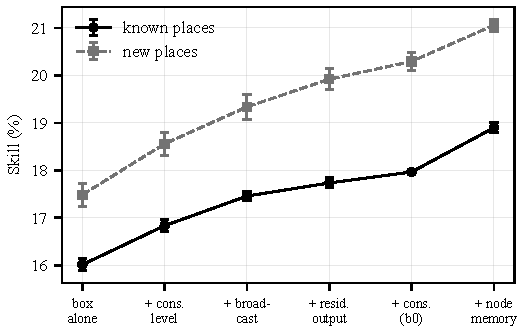
\includegraphics[width=\columnwidth]{figures/fig_stack.pdf}
\caption{Skill of the on-device model as components are added (mean over three seeds, bars show one standard deviation).}
\label{fig:stack}
\end{figure}

\subsection{Ablation of the Node Memory}
\label{sec:ablation}
\emph{1) Effectiveness of Surprise and Profile:} Table~\ref{tab:memory} separates the two inputs derived from the table. The surprise alone lowers the RMSE by 0.38\% at known and 0.61\% at new places, the profile alone by 0.56\% and 0.29\%, and both together by 1.09\% and 0.89\%. The two inputs carry different information, one about the present and one about the next hours, so the gain is larger than either one.

\emph{2) Is the Gain Specific to the Node:} A node memory could help only because it adds more inputs. In the placebo arm, every node reads the table of another node (node $i{+}7$), which has the same shape and statistics but the wrong site. It reaches 18.03\% against 17.97\% for the base, one sixth of the gain of the real table, and the real table is better than the placebo by 0.92\% (CI $-1.07$ to $-0.76$) at known and 0.77\% at new places. The pre-registered rule for this experiment asked for a gain of at least 0.3\%, a CI excluding zero, and a win over the placebo with a CI excluding zero; all three conditions held at known and new places.

\begin{table*}[!t]
\caption{Ablation of the Node Memory. Skill (\%, Mean $\pm$ Std over Three Seeds) and Change of RMSE (\%) With 95\% CI Against the Base Model in the First Row, Except in the Last Row}
\label{tab:memory}
\centering\footnotesize
\setlength{\tabcolsep}{3pt}
\begin{tabular}{|p{5.4cm}|c|c|c|c|}
\hline
Model & Known & New & $\Delta$RMSE known [CI] & $\Delta$RMSE new [CI] \\
\hline
Base (split-res + consensus) & 17.97$\pm$0.05 & 20.29$\pm$0.19 & reference & reference \\
+ surprise only & 18.24$\pm$0.08 & 20.74$\pm$0.24 & -0.38 [-0.47, -0.28] & -0.61 [-0.72, -0.49] \\
+ profile only & 18.46$\pm$0.07 & 20.56$\pm$0.11 & -0.56 [-0.67, -0.46] & -0.29 [-0.42, -0.16] \\
+ surprise and profile (node memory) & 18.90$\pm$0.11 & 21.06$\pm$0.13 & -1.09 [-1.27, -0.91] & -0.89 [-1.07, -0.70] \\
+ another node's table (placebo) & 18.03$\pm$0.02 & 20.31$\pm$0.24 & -0.17 [-0.23, -0.11] & -0.12 [-0.19, -0.05] \\
Node memory vs. placebo & & & -0.92 [-1.08, -0.76] & -0.77 [-0.96, -0.58] \\
\hline
\end{tabular}

\end{table*}

\subsection{Personal Forecasts and Message Budget}
A personal graph forecast sent every hour reaches a skill of 23.3\% on the saved unit-0 forecasts, against 15.7\% for the node alone. Fig.~\ref{fig:messages} shows what a limited number of messages buys. At 20\% of hours, the disagreement rule reaches 20.7\%, which is 66\% of the full cloud gain, while random sending reaches 17.1\%, 19\% of it. With a token bucket, four to six messages per node per day already give most of the benefit. A LightGBM model that learns when to send, trained on the first half of the test period and scored on the second half, improves on the simple rule by only 0.16 skill points at 20\% (threshold $+0.5$), and the difference stays small (Section~\ref{sec:other}), so the simple rule stays. When a personal forecast is one hour old, the path-based move with a fixed blend gives 19.4\%, against 15.9\% for the node; moving it against the sensor reading instead gives a skill of $-71\%$.

\begin{figure}[!t]
\centering
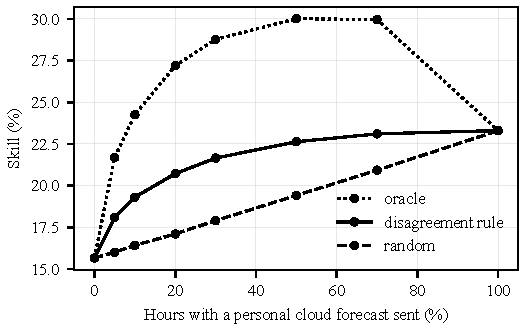
\includegraphics[width=\columnwidth]{figures/fig_messages.pdf}
\caption{Skill against the share of hours with a personal cloud forecast. The oracle sends in the hours where the cloud gains most.}
\label{fig:messages}
\end{figure}

\subsection{Stale and Missing Broadcasts}
A model trained and scored with a fresh broadcast is not safe when the link fails. We trained the split model with a random broadcast age of 0 to 6 hours and 15\% missing broadcasts and scored it at each age (Table~\ref{tab:stale}). Fresh, it reaches only 16.19\% for the three-hour broadcast, compared with 17.73\% for the same model trained with a fresh broadcast: the model cannot trust a message that is usually old, and most of the fresh gain is lost. A longer regional path of nine hours, shifted along by the node, helps when the broadcast is fresh (16.68\%), but at an age of three hours it keeps nothing over the node alone at known places. With the residual output, a missing broadcast sets $\hat R$ to zero, and the nine-hour model is then worse than the node alone: $+1.01\%$ (CI $+0.77$ to $+1.28$) at known and $+1.38\%$ at new places. The pre-registered rule asked for 40\% of the fresh gain at three hours and failed. A one-byte level broadcast with a plain input did not show this problem: it lowered the RMSE by 0.71\% when fresh and stayed within $\pm0.1\%$ of no broadcast when two or more hours old or missing. The no-regret property thus holds for the level only, and not for the full split model. We plan to test two models on the node, the split model while the broadcast is at most one hour old and the box-alone model otherwise.

\begin{table}[!htb]
\caption{Skill (\%) of the Split Model Trained for Random Broadcast Age, by Age of the Broadcast at Test Time (Hours; ``Miss.'' = No Broadcast)}
\label{tab:stale}
\centering\footnotesize
\setlength{\tabcolsep}{2.5pt}
\begin{tabular}{|l|p{2.1cm}|c|c|c|c|c|c|}
\hline
Places & Model & 0 & 1 & 2 & 3 & 6 & Miss. \\
\hline
Known & Box alone & 16.01 & 16.01 & 16.01 & 16.01 & 16.01 & 16.01 \\
Known & +1..+3 h broadcast & 16.19 & 15.82 & 15.98 & 16.01 & 15.99 & 16.00 \\
Known & +1..+9 h path & 16.68 & 16.19 & 16.12 & 15.99 & 15.73 & 15.42 \\
New & Box alone & 17.48 & 17.48 & 17.48 & 17.48 & 17.48 & 17.48 \\
New & +1..+3 h broadcast & 18.22 & 17.33 & 17.46 & 17.36 & 17.38 & 17.38 \\
New & +1..+9 h path & 18.59 & 17.93 & 17.84 & 17.72 & 17.39 & 16.59 \\
\hline
\end{tabular}

\end{table}

\subsection{Other Tests}
\label{sec:other}
Table~\ref{tab:other} collects the remaining comparisons. A loss that penalises a wrong direction, and a loss that weights errors near the CPCB category limits, were both worse than the Huber loss on the score they were meant to help. A fuzzy Takagi-Sugeno gate in place of the dense head equals the model without it (skill 15.89\% against 16.02\%) and is useful only for readability. Weather inputs on the node gave no gain. An exhaustive search over all 128 subsets of the seven optional sensors with a LightGBM probe puts the core set (PM, humidity and temperature, clock) at 17.74\% for 0.55 W, adds 0.68 skill points for the two fans, and 0.33 for the MQ-7; the MQ-135 adds 0.05 for about 0.8 W (power values still need verification on hardware).

\begin{table}[!htb]
\caption{Other Comparisons: Change of RMSE (\%) With 95\% CI at Known Places}
\label{tab:other}
\centering\footnotesize
\setlength{\tabcolsep}{3pt}
\begin{tabular}{|p{4.0cm}|c|c|}
\hline
Comparison & $\Delta$RMSE [CI] & Result \\
\hline
Trend loss (hinge on wrong direction) vs. Huber & +0.64 [+0.41, +0.87] & worse \\
AQI-breakpoint weighted loss vs. Huber & +0.38 [+0.22, +0.54] & worse \\
1 M training windows vs. 200 k & -1.06 [-1.30, -0.81] & better \\
Width 64 vs. width 32 (1 M windows) & +0.06 [-0.08, +0.20] & no difference \\
Learned send rule vs. disagreement rule (20\% sent) & -0.20 [-0.34, -0.05] & below threshold \\
\hline
\end{tabular}

\end{table}

\section{Analysis and Discussion}
\label{sec:discussion}
\subsection{What Each Part Contributes and Why}
The results separate two kinds of information. The broadcast carries what all nodes share, and a single noisy node cannot observe it well, so sending it gives the largest step. The node memory carries what is private to the node and repeats daily, which neither a 24-hour window nor the cloud forecast provides, and the placebo shows that the gain comes from the site and not from extra inputs. This is the opposite of the setting in the distillation papers we started from \cite{na2026privileged,fu2026rednet}, where the large model sees the same data. Table~\ref{tab:position} states the difference. In those works a gap in capacity is closed by training. Here the gap is in information, and it is closed at run time, with eight bytes.

\begin{table*}[!t]
\caption{Position of SplitMem Against the Edge-Forecasting Works That Use a Teacher-Student Setting}
\label{tab:position}
\centering\footnotesize
\setlength{\tabcolsep}{3pt}
\begin{tabular}{|l|l|l|l|}
\hline
Work & What the large model has that the small one lacks & How it reaches the small model & Task \\
\hline
Na et al.~\cite{na2026privileged} & greater capacity; privileged information in training & distillation losses at training time & on-device time series \\
REDNet~\cite{fu2026rednet} & pre-trained foundation model, more robust & two-stage distillation & edge time series \\
KDAQnet~\cite{kumar2026kdaqnet} & larger network on satellite data & distillation & multi-pollutant forecasting \\
Shmuel et al.~\cite{shmuel2026forest} & higher accuracy (boosting) & student fits the teacher output & symbolic regression \\
\hline
SplitMem (this work) & data of all other nodes at run time & broadcast input (8 B) + node memory; no copying & PM change of a low-cost node \\
\hline
\end{tabular}
\end{table*}

\subsection{Why Wind Direction Does Not Help Here}
The placebo-controlled test is a negative result and we report it as one. ERA5 has only four distinct wind series for 32 stations, the measured vanes are noisy, Delhi behaves as one airshed (one cluster of 28 stations by the correlation of 3 h changes, with within-cluster correlation 0.33 and between-cluster 0.10), stations are 5 to 15 km apart so that air needs one to four hours to cross at winter wind speeds, and the wind speed is already available from the fans and from ERA5. Denser nodes or longer horizons may change this, and we do not claim that wind direction never matters.

\subsection{On-Device Deployment}
The node model is below 15\,000 parameters in the context-only form, and the extra state is 48 table entries and a few multiplications per hour. Two models of about 60 KB each fit in the flash of the ESP32 for the planned two-model fallback. The firmware for sensing and the hourly feature code exists and is checked against the notebooks; receiving the broadcast, the consensus and memory update, and holding two models are not built yet.

\subsection{Limitations and Threats to Validity}
All results use simulated sensors, so the simulator decides how informative each sensor and node is, and every number needs confirmation with real nodes co-located with a CPCB station. With an uncalibrated sensor the CPCB category of the shown level is right only 43\% of the time (71\% from the true level), so the level needs calibration. The cloud graph model uses hindcast weather; live forecasts will be about one point worse, up to three at six hours, while the regional forecaster and the node use no future weather. The nodes are at station places, 5 to 15 km apart, and a real network may be denser or sparser. The broadcast was built from 27 nodes, and the effect of fewer nodes is not tested. The memory and the consensus level use the node's own PM reading, so a faulty particle sensor affects them too. The learned send rule was fitted and scored inside the test period because no 2024 forecasts were saved. The training-size study used two seeds, and the node models in the stack used 200\,000 of 2.6 M training windows, so the stack should grow when trained on 1 M windows; a final run with all components and a direct bootstrap of the full stack against the box-alone model is planned. Finally, the idea of a global forecast corrected by a local model exists in hierarchical forecasting and in model output statistics. We therefore claim the form for byte-limited nodes and microcontroller models, the node memory with its placebo control, and the measured behaviour under link failure, and we make no claim of being first.

\section{Conclusion}
\label{sec:conclusion}
In this article, we presented SplitMem, a cloud-assisted forecaster for low-cost PM nodes. The cloud broadcasts the city-wide change in eight bytes per hour, and the on-device model predicts only its local correction, helped by a table of its own usual offset at each clock hour. On simulated nodes in Delhi-NCR the stack lowered the RMSE of the on-device forecast by about 3.4\% at known places and 4.3\% at new places compared with the model alone, and a placebo test showed that the memory gain belongs to the node. A disagreement-triggered personal forecast gave two thirds of the full cloud gain with one fifth of the messages. Copying the cloud model into the node had added little, because the cloud lead comes from information the node cannot see. The negative results, wind direction, learned sending, buffered broadcasts and training for stale links, show where the design stops. Future work is to run the final stack on 1 M windows, to test the two-model fallback and the number of nodes needed, to test faulty sensors, and above all to co-locate real nodes with a reference station.

\section*{Acknowledgment}
The authors thank the Central Pollution Control Board for the open station data and Open-Meteo for the ERA5 access. [AI-assistance disclosure to be completed according to the policy of the target venue.]

\FloatBarrier
\bibliographystyle{IEEEtran}
\bibliography{refs}
\end{document}
